En la revisión de literatura, podemos encontrar el simulador 
"Lunar Phase Simulator" de la Universidad de Nebraska-Lincoln’s. \cite{Ucar2014}

\begin{figure}[h]
    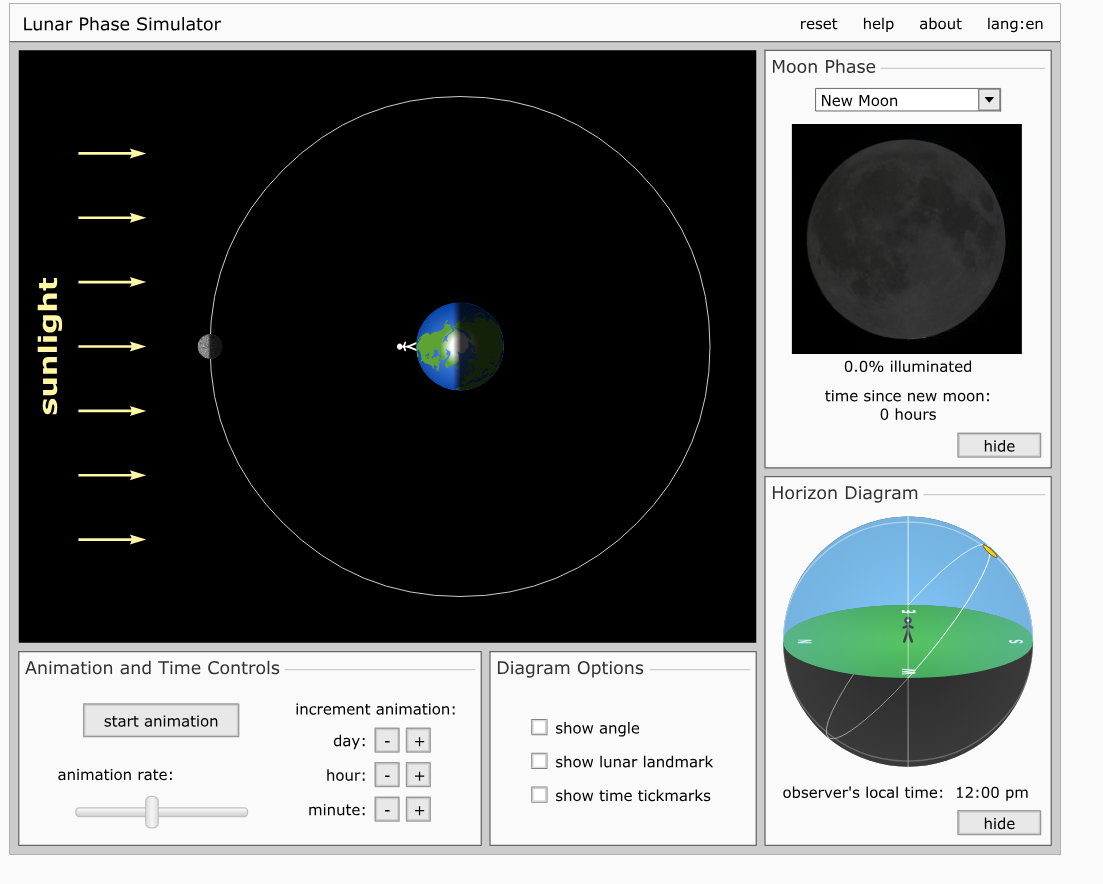
\includegraphics[scale = 0.5]{Imagenes/nebraska.png}
    \centering
    \caption{Simulador de fases de la luna}{Fuente: \cite{UNL2025}}
\end{figure}

\vspace{2em}
El simulador permite a los estudiantes comprender visualmente cómo la Luna cambia de fase al orbitar la Tierra, mostrando la relación entre la posición de la Luna, la Tierra y la luz solar. Para lograrlo, se emplea un frontend desarrollado con HTML, JavaScript y CSS, que incluye controles interactivamente ajustables para modificar el tiempo y observar en tiempo real el cambio de fases.

La representación visual abarca una simulación orbital en 2D, una vista desde el horizonte del observador y un indicador de fase lunar que muestra el porcentaje de iluminación. Como resultado, este recurso se presenta como una herramienta intuitiva y visualmente atractiva para la enseñanza en todos los niveles, no requiere conocimientos previos al basarse en la manipulación gráfica y resulta ideal para principiantes en astronomía.

\addcontentsline{toc}{subsection}{Análisis comparativo}
\subsection*{Análisis comparativo}

A continuación, se realiza una comparativa del simulador de la figura 5 con nuestra propuesta del prototipo:

\begin{table}[H]
    \centering
    \begin{tabular}{|p{4.5cm}|p{5.5cm}|p{5.5cm}|}
        \hline
        \textbf{Criterio} & \textbf{Lunar Phase Simulator (Nebraska)} & \textbf{Propuesta} \\
        \hline
        \textbf{Objetivo} & Visualizar fases lunares de forma interactiva. & Simulación científica con datos reales, material descargable y evaluación del aprendizaje. \\
        \hline
        \textbf{Interactividad} & El usuario ajusta la posición de la Luna manualmente. & El usuario ingresa fechas, obtiene gráficos y responde un \textbf{quiz interactivo} para reforzar el aprendizaje. \\
        \hline
        \textbf{Datos Adicionales} & No proporciona información numérica. & Muestra distancia Tierra-Luna, iluminación y visibilidad, además de permitir la autoevaluación. \\
        \hline
        \textbf{Exportación de Datos} & No permite guardar información. & Genera reportes en PDF para estudiantes con sus resultados del quiz y gráficos de fases lunares. \\
        \hline
        \textbf{Aplicabilidad Educativa} & Bueno para principiantes en astronomía. & Útil tanto para estudiantes como para investigadores, incorporando \textbf{evaluación y retroalimentación} del aprendizaje. \\
        \hline
    \end{tabular}
    \caption{Comparación entre el Lunar Phase Simulator (Nebraska) y la propuesta del prototipo, incluyendo evaluación interactiva.}
    \label{tab:comparacion}
\end{table}
